\begin{solution}{normal}
Let the diode have a potential difference (p.d.) of $V$. By idea 24, it is quite apparent that the p.d. across the reistor will be 
\[1.5 - V = I r.\]
Taking $i$ to be in mA which means $i = 1000 I$, we find that 
\[i (V) = 15 - 10 V.\]
We also have the equation of the current voltage graph $I(V)$, which allows to find the intersection between this line and the graph. 
\begin{center}
    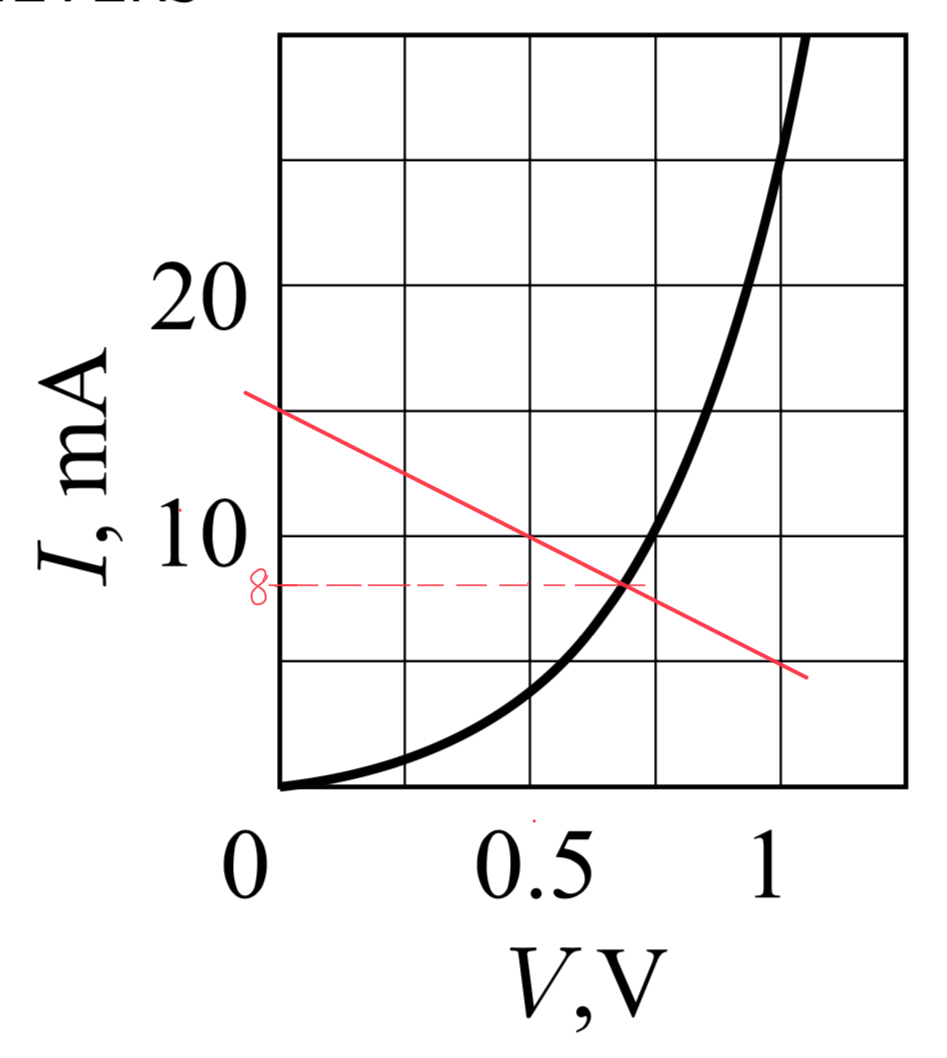
\includegraphics[width=7cm]{49B62025-1343-4881-9854-3AF244D6DE23.jpeg}
\end{center}
\end{solution}